\documentclass[a4paper, 10pt]{article}

%Internal Packages
\usepackage[utf8]{inputenc}
\usepackage[french]{babel}
\usepackage[T1]{fontenc}
\usepackage{graphicx}
\usepackage{hyperref}       % Pour les liens hypertextes

%Variables
\title{Rapport de projet : CoreWar}
\author{Amand Henry\and{}Théo Sicot\and{}Etienne Bossu\and{}Tom Rousée}
\date{\today{}}

%Document
\begin{document}
    \maketitle{}
    \newpage{}
    \tableofcontents{}
    \newpage{}

    % Introduction
    \begin{section}{Introduction} \label{sec:introduction}
        \par
            Le \textbf{Corewar} est un jeu de programmation créer en 1984 dans les universités américaines où deux programmes sont opposés pour prendre le contrôle d'une machine virtuelle appelée \textbf{MARS} (Memory Array Redcode Simulator). Ces programmes sont écrits dans un langage proche de l'assembleur appelé \textbf{RedCode}. L'intérêt de ce langage est qu'il n'est pas compris par les ordinateurs, il y a donc peu de risque qu'ils s'échappent de la machine et qu'il cause des problèmes dans le pc des joueurs. Les programmes, appelés "Guerriers", ont pour objectif d'être les derniers à s'exécuter en faisant se terminer toutes les instances du programme adverse.
            \bigskip
        \par
            Au début les joueurs concevaient leurs programmes par eux mêmes mais avec la popularisation des \textbf{algorithmes génétiques}, beaucoup utilisent l'ordinateur pour essaier de trouver les meilleurs programmes possible et gagner la partie.
            \bigskip
        \par
            Dans ce projet nous devions créer tout ce qu'il y a besoin pour faire une partie de CoreWar : la machine MARS, l'interpréteur pour le RedCode ainsi qu'un algorithme génétique qui permet de créer des guerriers efficaces. 
            \bigskip
        \par
            Ce rapport commencera par une présentation détaillé du projet, puis nous expliquerons les fonctionnalités implémentées, les éléments techniques utilisés ainsi que les choix de conception que nous avons fait. Ensuite nous présenterons les résultats obtenus. Enfin nous conclurons sur ce que nous avons appris et les perspectives futures.
    \end{section}

    % Méthodologie
    \begin{section}{Le projet} \label{sec:projet}
        
        \subsection{Objectifs}
            \par
                L'objectif de ce projet était de créer un jeu de CoreWar complet. Pour cela nous avons dû identifier les points principaux qui composent notre projet et les implémenter. Nous avons donc décidé de découper notre projet en plusieurs parties :
                \smallskip
                \begin{enumerate}
                    \item La machine MARS
                    \item Le RedCode
                    \item Un algorithme génétique pour créer des guerriers
                    \item Une interface graphique pour afficher le déroulement des parties
                \end{enumerate}
                \medskip
                Nous avions pour la réalisation de ce projet un peu plus de 3 mois. Durée de temps appropriée car elle nous a permis de bien réfléchir aux détails de la création du jeu et de le réaliser dans les temps sans avoir a délaisser les autres cours.
                \bigskip

        
        \begin{subsection}{Machine MARS}
            \par
                La \textbf{machine MARS} est la pièce maitresse des parties de CoreWar. C'est la machine virtuelle dans laquelle les guerriers vont s'exécuter. Elle gère la mémoire, le RedCode et le déroulement des parties. 
                \medskip
            \par
                La principale problèmatique de cette partie était la \textbf{représentation de la mémoire}.
                Nous avons choisit d'utiliser une \textbf{liste chainée} car la mémoire devait être circulaire et cette structure de données permet de facilement la parcourir en boucle, chaque cellule connaissant la suivante et la précédente. Il suffisait de faire pointer la dernière cellule vers la première pour avoir une liste circulaire.
                Dans cette liste chainée chaque cellule contient \textbf{une instruction et deux Operande}. Les instructions sont des commandes en RedCode qui permettent de déplacer les guerriers, de modifier la mémoire, de sauter des instructions, etc. Les opérandes sont quant à eux un couple valeur-mode qui associe un entier et le mode d'adressage de cette valeur (Direct, Indirect, Immédiat et Pre-Decrement). Nous reviendrons sur ces différents modes d'adressage et instructions dans la partie sur le RedCode.
                \medskip
            \par
                La machine MARS doit aussi gérer le déroulement de la partie. L'idée est que chaque guerrier exécute chacun à son tour une instruction. Pour cela elle a aussi à sa disposition une liste des instructions à exécuter, qui est en fait une liste de certaines cellules de la mémoire (celles dans lesquelles un guerrier à une opération en cours). Cela permet de facilement déterminer quel guerrier doit jouer et de lui faire exécuter son instruction au bon moment.
        \end{subsection}

        \begin{subsection}{Détails du RedCode : Langage et Interpréteur}
            \par
                Le \textbf{RedCode} est un langage proche de l'assembleur qui permet de programmer les guerriers. (Pour ce projet nous utilisons la norme icw88.) Il est composé de 11 instructions. Chaque instruction est associée à deux opérandes qui définissent les valeurs sur lesquelles l'instruction va s'appliquer. Chacun de ces opérandes peuvent être de 4 types / modes d'adressages différents : \textbf{Direct, Indirect, Immédiat et Pre-Decrement}.
                \bigskip \newline
                    \textit{Voici les différentes instructions et leurs effets :}
                \bigskip

                \begin{tabular}{|c|p{8cm}|}
                    \hline
                        \textbf{Instruction} & \textbf{Description} \\
                    \hline
                        DAT A B & Supprime le processus en cours d'exécution de la file d'attente des processus \\
                    \hline
                        MOV A B & Déplace A dans B \\
                    \hline
                        ADD A B & Ajoute A à B \\
                    \hline
                        SUB A B & Soustrait A à B \\
                    \hline
                        JMP A B & Saute à A \\
                    \hline
                        JMZ A B & Saute à A si B est égal 0\\
                    \hline
                        JMN A B & Saute à A si B est différent de 0 \\
                    \hline
                        CMP A B & Si A est égal à B, ignore l'instruction suivante\\
                    \hline
                        SLT A B & Si A est inférieur à B, ignore l'instruction suivante\\
                    \hline
                        DJN A B & Décrémente B; Si B est différent de 0, saute à A \\
                    \hline
                        SPL A B & Place A dans la file d'attente des processus \\
                    \hline
            \end{tabular}

            \bigskip
            Chacune de ces instructions peut être utilisée avec les 4 modes d'adressages différents. Ces modes d'adressages permettent de définir comment l'opérande doit être utilisé.
            \bigskip \newline
                \textit{Voici les différents modes d'adressage et leurs effets :}
            \bigskip

            \begin{tabular}{|c|p{8cm}|}
                \hline
                    \textbf{Mode} & \textbf{Description} \\
                \hline
                    Direct & L'opérande est une adresse mémoire \\
                \hline
                    Indirect & L'opérande est une adresse mémoire vers une autre cellule dont on utilise l'operande B \\
                \hline
                    Immédiat & L'opérande est une valeur \\
                \hline
                    Pre-Decrement & TODO : A Compléter\\
                \hline
            \end{tabular}
        \end{subsection}




        \begin{subsection}{Algorithme Génétique}
            \begin{subsubsection}{Fonctionnement}
                Description de l'algorithme génétique utilisé pour créer des guerriers.
            \end{subsubsection}

            \begin{subsubsection}{Entrainement}
                Description des méthodes utilisées pour l'entrainement des guerriers.
            \end{subsubsection}
        \end{subsection}



        \begin{subsection}{Interface Graphique}
            \par
                L'interface graphique permet de visualiser le déroulement des parties de CoreWar. Elle affiche la mémoire et les guerriers qui s'affrontent dedans.
                Elle se lance au choix de l'utilisateur et permet de visualiser une partie en cours. 
                \smallskip
            \par
                Toute l'interface a été faite avec le package \textbf{swing}, déjà inclus dans java. Elle transforme la mémoire en une grille. Cette grille s'adapte à toute les tailles de mémoire pour d'éventuelles parties sur une mémoire a taille réduite. Elle est composée de cases qui peuvent être de 3 couleurs différentes : Bleu, Rouge et Noir. (le Bleu et le Rouge pour chacun des guerriers et le Noir pour les cases qui n'appartiennent encore a personne).
                \bigskip
            
                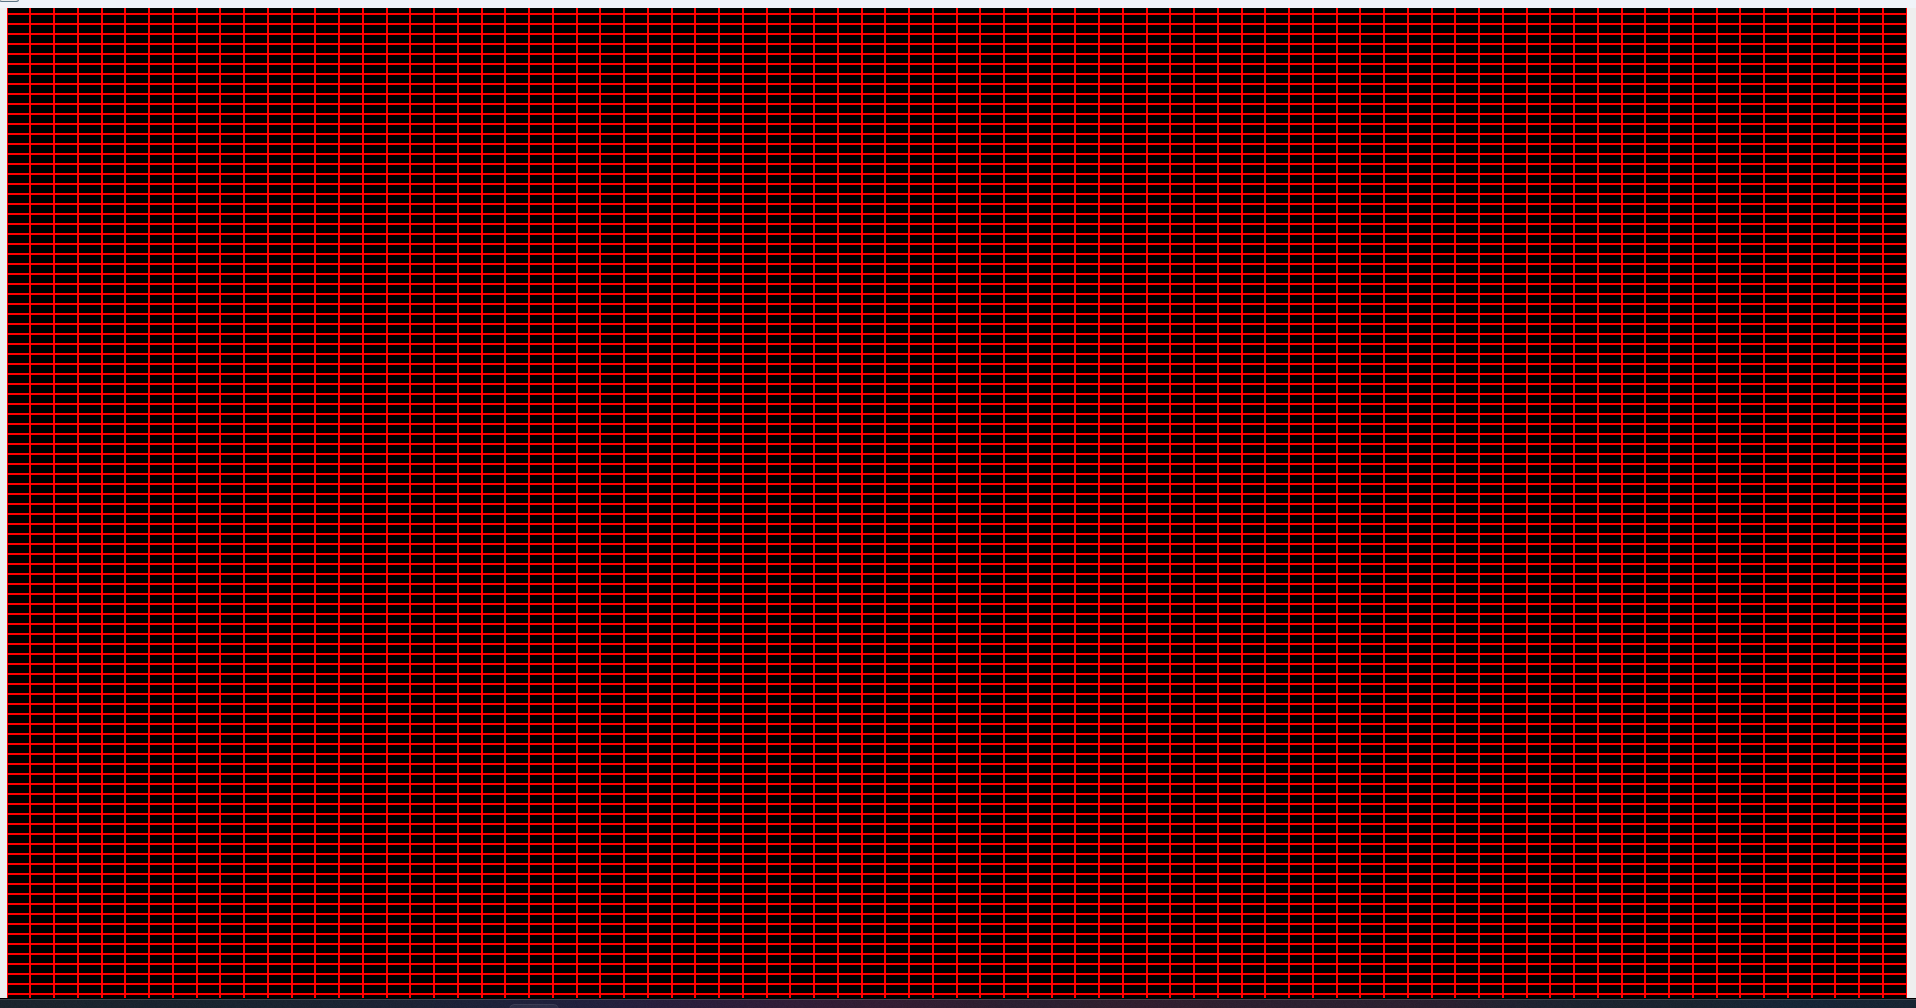
\includegraphics[width=10cm]{img/grille_interface.png}\newline
                \textit{La grille de 8000 cases, taille la plus courante pour les parties de CoreWar.}
                \bigskip

            \par
                Pour l'affichage final on efface les bordures pour afficher uniquement les couleurs. Cela permet de mieux visualiser les guerriers et de ne pas être gêné par les bordures.
                \bigskip

                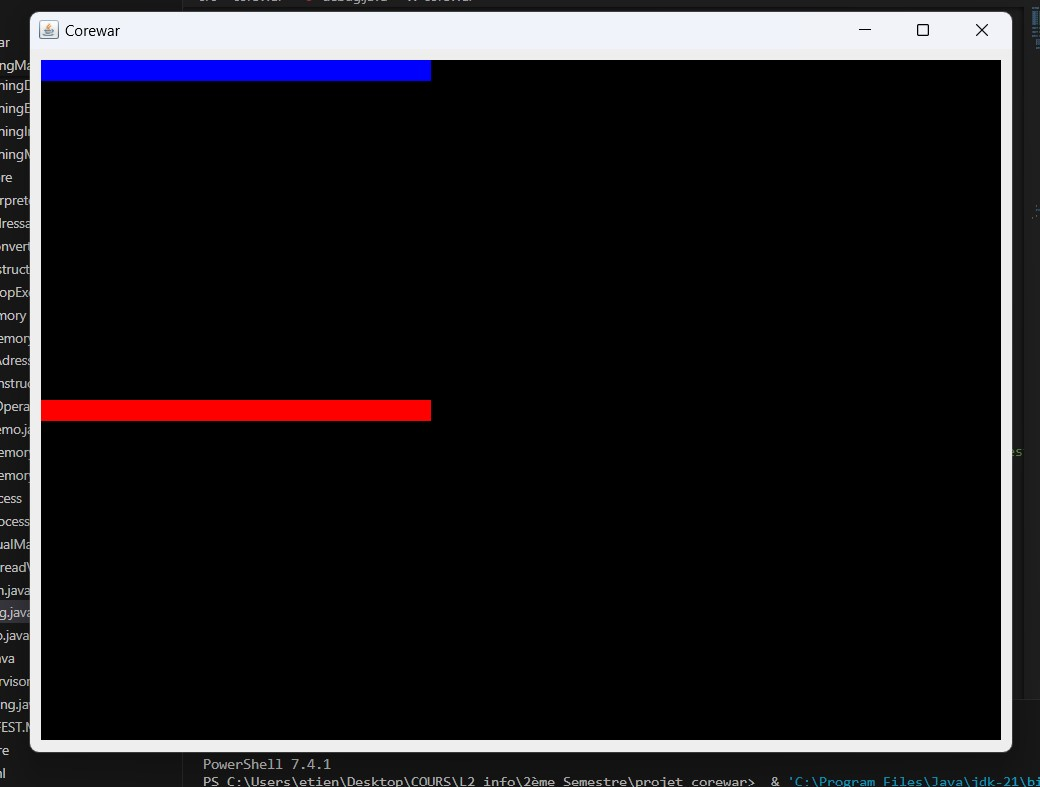
\includegraphics[width=10cm]{img/display.jpg}\newline
                \textit{Affichage final de l'interface graphique. Sans les bordures durant une partie.}
                \bigskip
            
            \par
                Pour actualiser l'affichage plusieurs méthodes ont été créées. Au départ la méthode consistait a prendre une nouvelle grille et à remplacer l'ancienne par la nouvelle. Mais cela ralentissait énormément l'affichage. Nous avons donc décidé de créer une méthode qui actualise uniquement les cases qui ont changé de couleur. Cela a permis d'optimiser l'affichage et de ne pas ralentir le jeu.
                Pour ce faire l'utilisation d'un GridBagLayout plutôt qu'un GridLayout simple a été nécessaire et il a fallu recréer l'interface. Dorénavant chaque case est gérée comme un élément indépendant et peut être actualisée indépendamment des autres.
        \end{subsection}
    
    \end{section}


    \begin{section}{Architecture du projet}\label{sec:architecture}
        \begin{subsection}{Diagramme de classe}
            \par
                Insérer des diagramme de classe du projet et les expliquer.
        \end{subsection}
    \end{section}

    \begin{section}{Résultats}\label{sec:resultats}
        Présentez les résultats obtenus, avec éventuellement des captures d'écran du jeu en action, des graphiques de performances, etc.
    \end{section}

    % Conclusion
    \begin{section}{Conclusion}\label{sec:conclusion}
        Résumer les résultats, ce qu'on a appris durant le projet, et les perspectives futures.
    \end{section}

    % Références
    \bibliographystyle{plain}
    \bibliography{references}
    
\end{document}